\section{Gerichtete Graphen}
\begin{itemize}
    \item Graph, dessen Kanten alle gerichtet sind
    \item Digraph ist: G = (V,E)
    \item Wenn G einfach ist: m < n(n-1)
    \item Wenn In- und Out-Kanten in separaten Adjazenz- Listen sind: Laufzeit für Zugriff auf In- und Out-Kanten proportional zur Grösse der Listen
\end{itemize}

\subsection{Gerichtete Tiefensuche}
\begin{itemize}
    \item DFS und BFS für Digraphen spezialisieren, indem Kanten nur entlang ihrer Richtung traversiert werden
    \item Im gerichteten DFS-Algorithmus haben wir vier Typen von Kanten:
\end{itemize}
\vspace{-8pt}
\begin{center}
    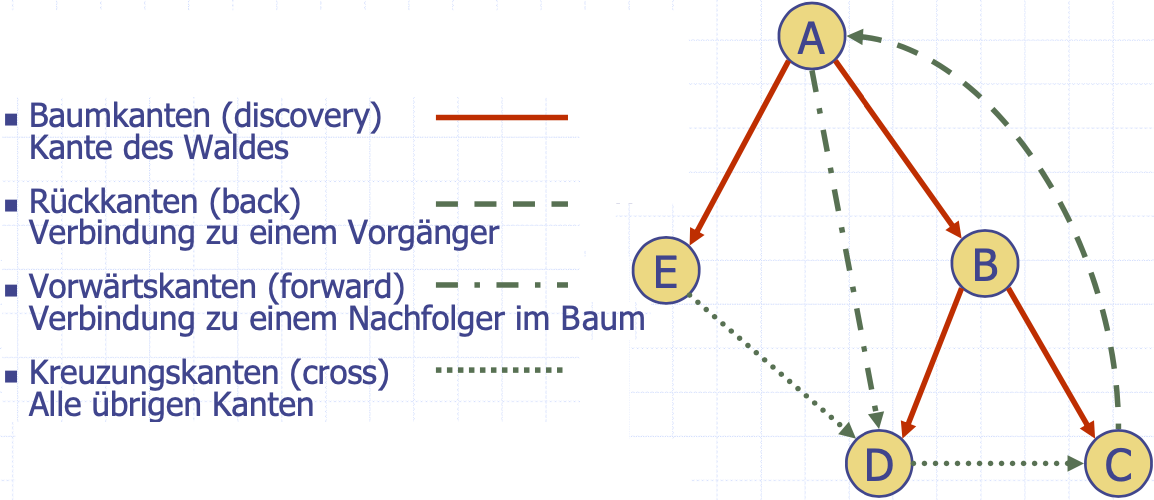
\includegraphics[scale=.28]{graphic/14 Digraphs/Gerichtete Tiefensuche.png}
\end{center}
\vspace{-8pt}
Eine gerichtete Tiefensuche beginnt bei einem Vertex s und bestimmt die Vertizes, welche von s aus erreichbar sind

\subsection{Erreichbarkeit}
DFS Baum mit Wurzel v : Vertizes erreichbar von v durch gerichtete Pfade
\vspace{-8pt}
\begin{center}
    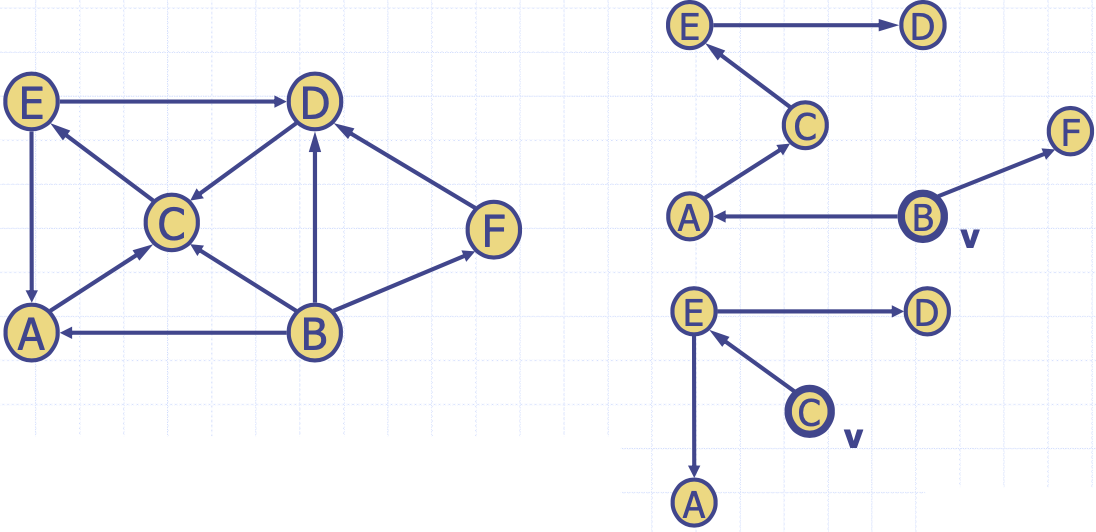
\includegraphics[scale=.22]{graphic/14 Digraphs/Erreichbarkeit.png}
\end{center}
\vspace{-8pt}

\subsection{Strong Connectivity}
Jeder Vertex kann alle anderen Vertizes erreichen
\subsubsection{Algorithmus}
\begin{itemize}
    \item Wähle einen Vertex v in G
    \item Führe eine Tiefensuche von v in G durch
    \begin{itemize}
        \item wenn es einen nicht besuchten Vertex w gibt: return false
    \end{itemize}
    \item G’ sei G mit umgekehrten Kanten (Richtungen)
    \item Führe eine Tiefensuche durch von v in G’
    \begin{itemize}
        \item wenn es einen nicht besuchten Vertex w gibt: return false
        \item sonst: return true //OK
    \end{itemize}
\end{itemize}
Laufzeit: O(n+m)

\subsection{Streng verbundene Komponenten}
\begin{itemize}
    \item Maximaler Subgraph, sodass jeder Vertex alle anderen Vertizes im Subgraph erreichen kann
    \item Laufzeit: O(n+m) mit Tiefensuche, ist aber komplizierter (ähnlich zu Biconnectivity)
\end{itemize}
\vspace{-8pt}
\begin{center}
    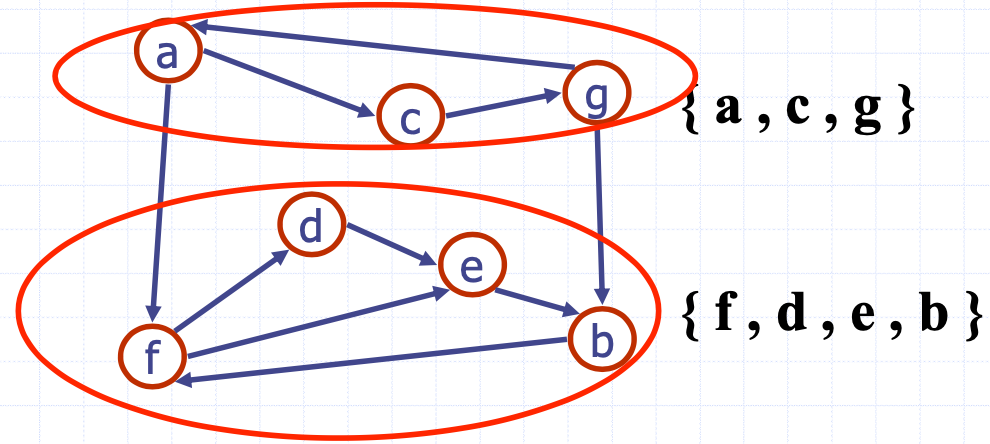
\includegraphics[scale=.2]{graphic/14 Digraphs/Streng verbundene Komponenten.png}
\end{center}
\vspace{-8pt}

\subsection{Transitiver Abschluss}
Laufzeit: O(n(n+m))
\vspace{-8pt}
\begin{center}
    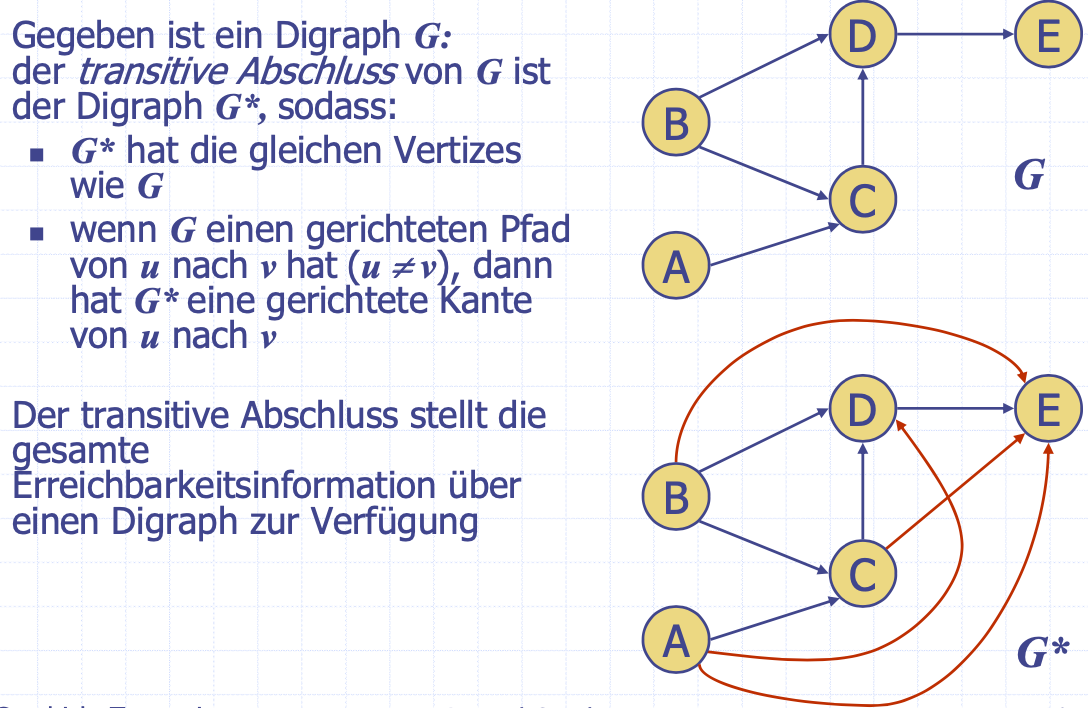
\includegraphics[scale=.28]{graphic/14 Digraphs/Transitiver Abschluss.png}
\end{center}
\vspace{-8pt}

\subsection{Floyd-Warshall Algorithmus}

\begin{center}
    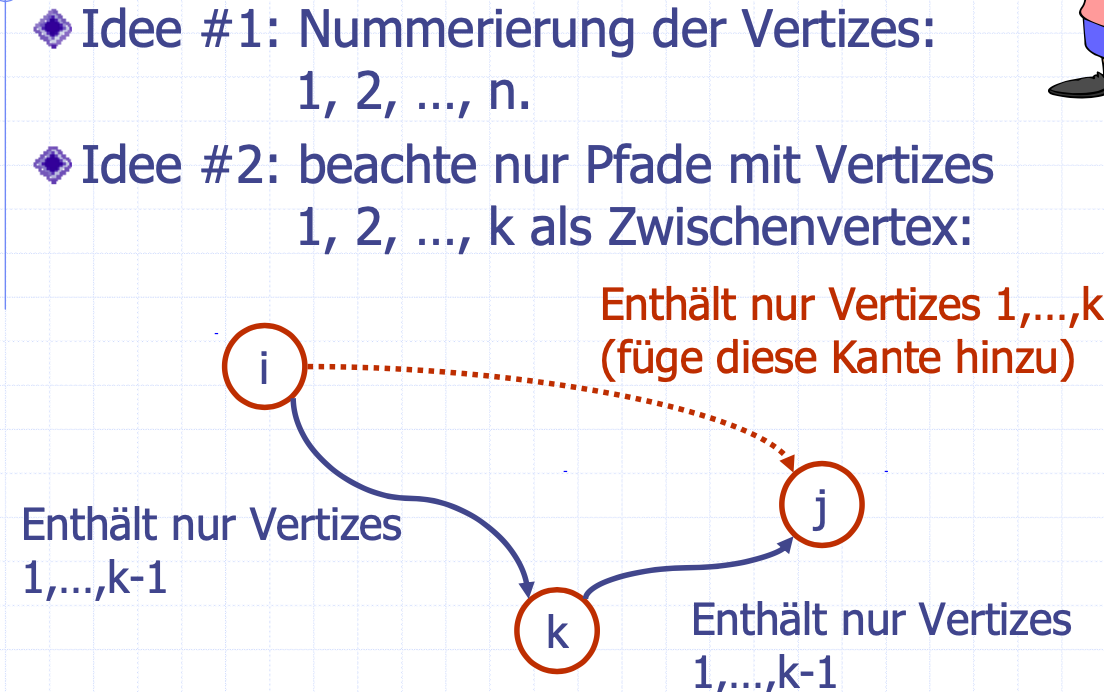
\includegraphics[scale=.22]{graphic/14 Digraphs/Floyd-Warshall Algorithmus.png}
    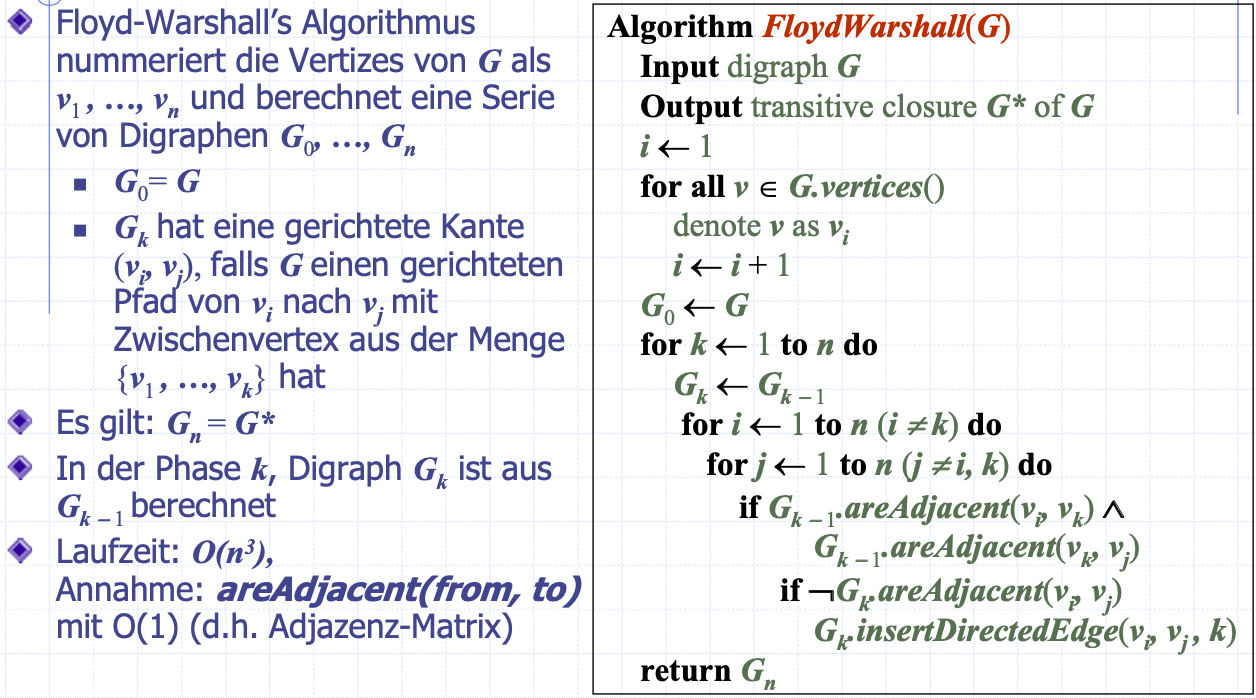
\includegraphics[scale=.28]{graphic/14 Digraphs/Floyd-Warshall Algorithmus2.png}
    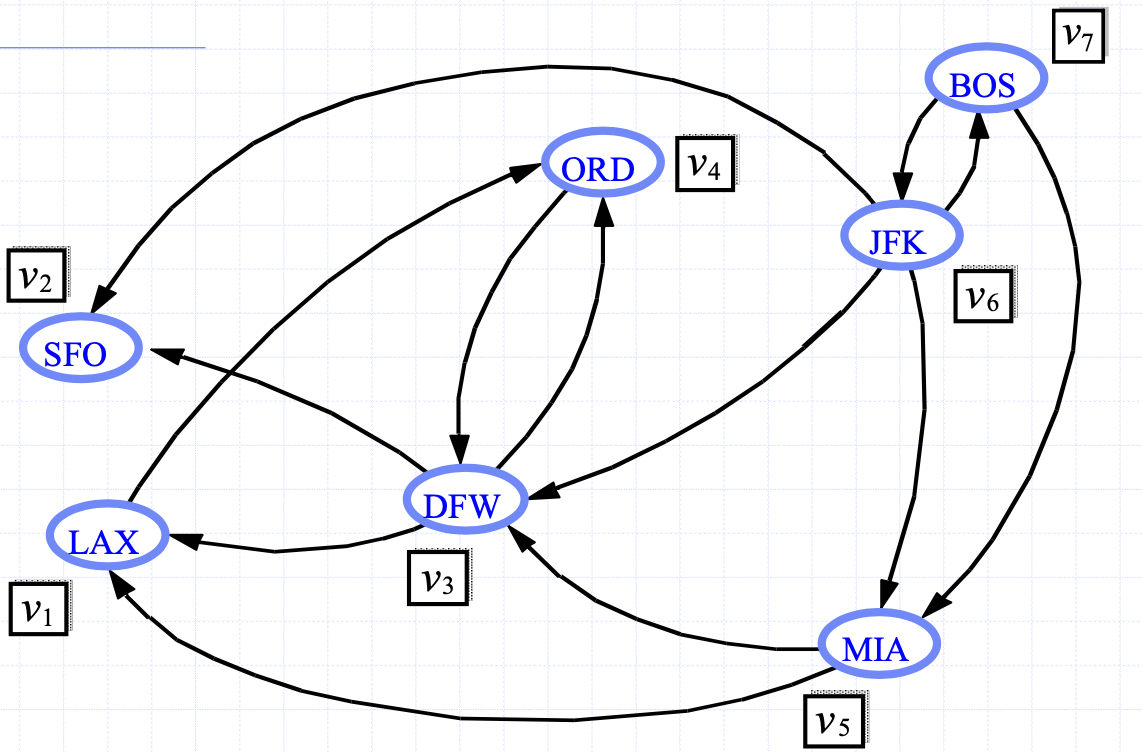
\includegraphics[scale=.22]{graphic/14 Digraphs/Floyd-Warshall Algorithmus3.png}
\end{center}
\vspace{-8pt}

\subsection{DAG’s und topologische Ordnung}
\begin{itemize}
    \item gerichteter azyklischer Graph (Directed Acyclic Graph (DAG)) ist ein Digraph, der keine gerichtete Zyklen enthält
    \item Eine topologische Ordnung eines Digraphs ist definiert durch die Nummerierung: $v_1 , ..., v_n$ der Vertizes, sodass für jede Kante ($v_i , v_j$) gilt: i < j
\end{itemize}
\vspace{-8pt}
\begin{center}
    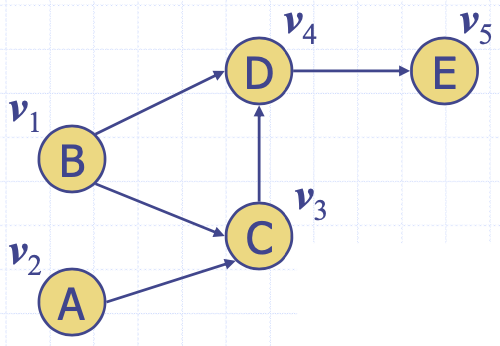
\includegraphics[scale=.25]{graphic/14 Digraphs/DAG.png}
\end{center}
\vspace{-8pt}
\subsubsection{Topologische Sortierung}
Laufzeit: O(n + m)
Nummeriere Vertizes, sodass für (u,v) in E gilt: u < v
\vspace{-8pt}
\begin{center}
    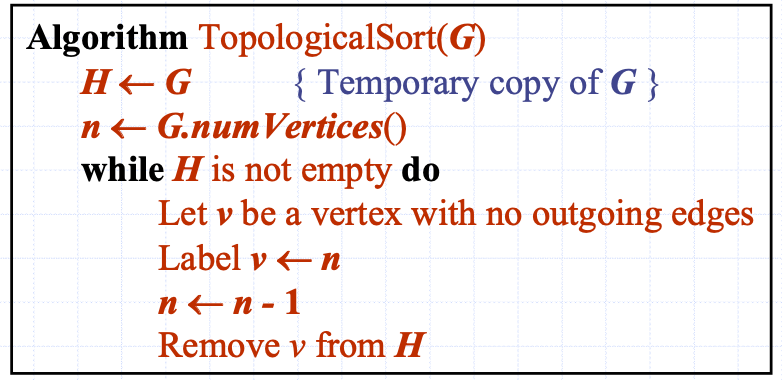
\includegraphics[scale=.28]{graphic/14 Digraphs/topologische Sortierung.png}
\end{center}
\vspace{-8pt}
\subsubsection{Topologische Sortierung mit Tiefensuche}
\begin{center}
    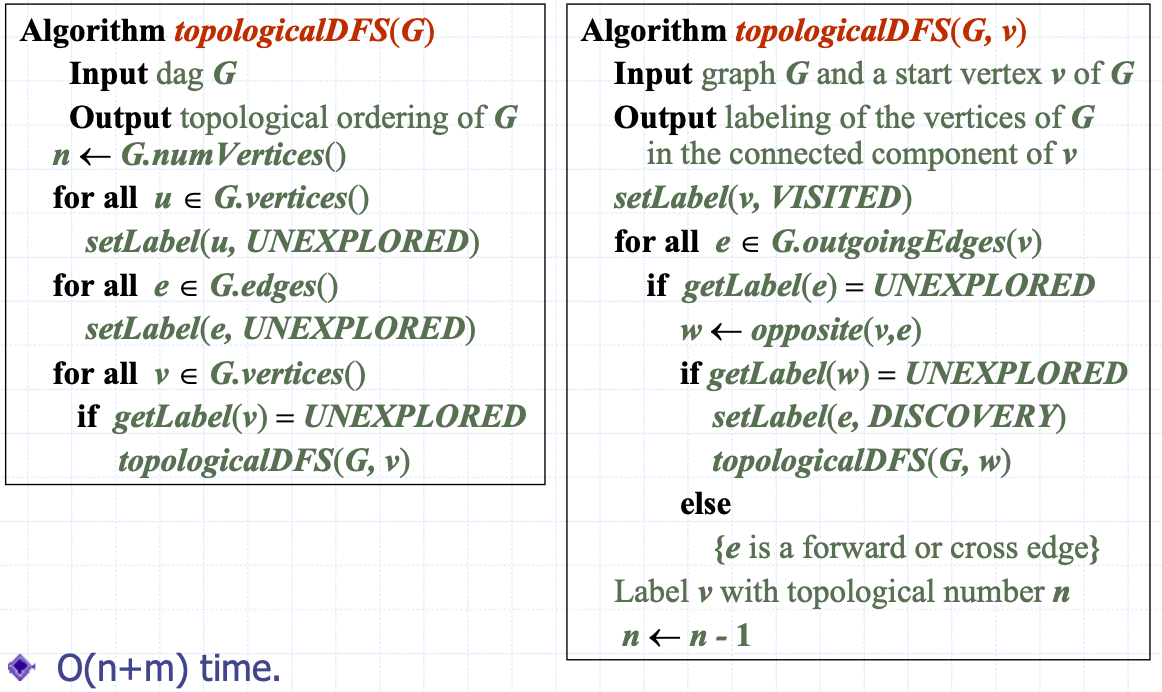
\includegraphics[scale=.28]{graphic/14 Digraphs/topologische Sortierung mit Tiefensuche.png}
\end{center}
\vspace{-8pt}

\vfill
$ $
\columnbreak
\paragraph{Floyd-Warshall}
Es gibt 3 verschiedene for-Schlaufen\\

Besteht eine Verbindung von Knoten i $\rightarrow$ k $\rightarrow$ j, dann:\\
Neue Verbindung von i $\rightarrow$ j

k ist oberste Schleife\\
i ist mitlere Schleife\\
j ist unterste Schleife\\

\begin{center}
    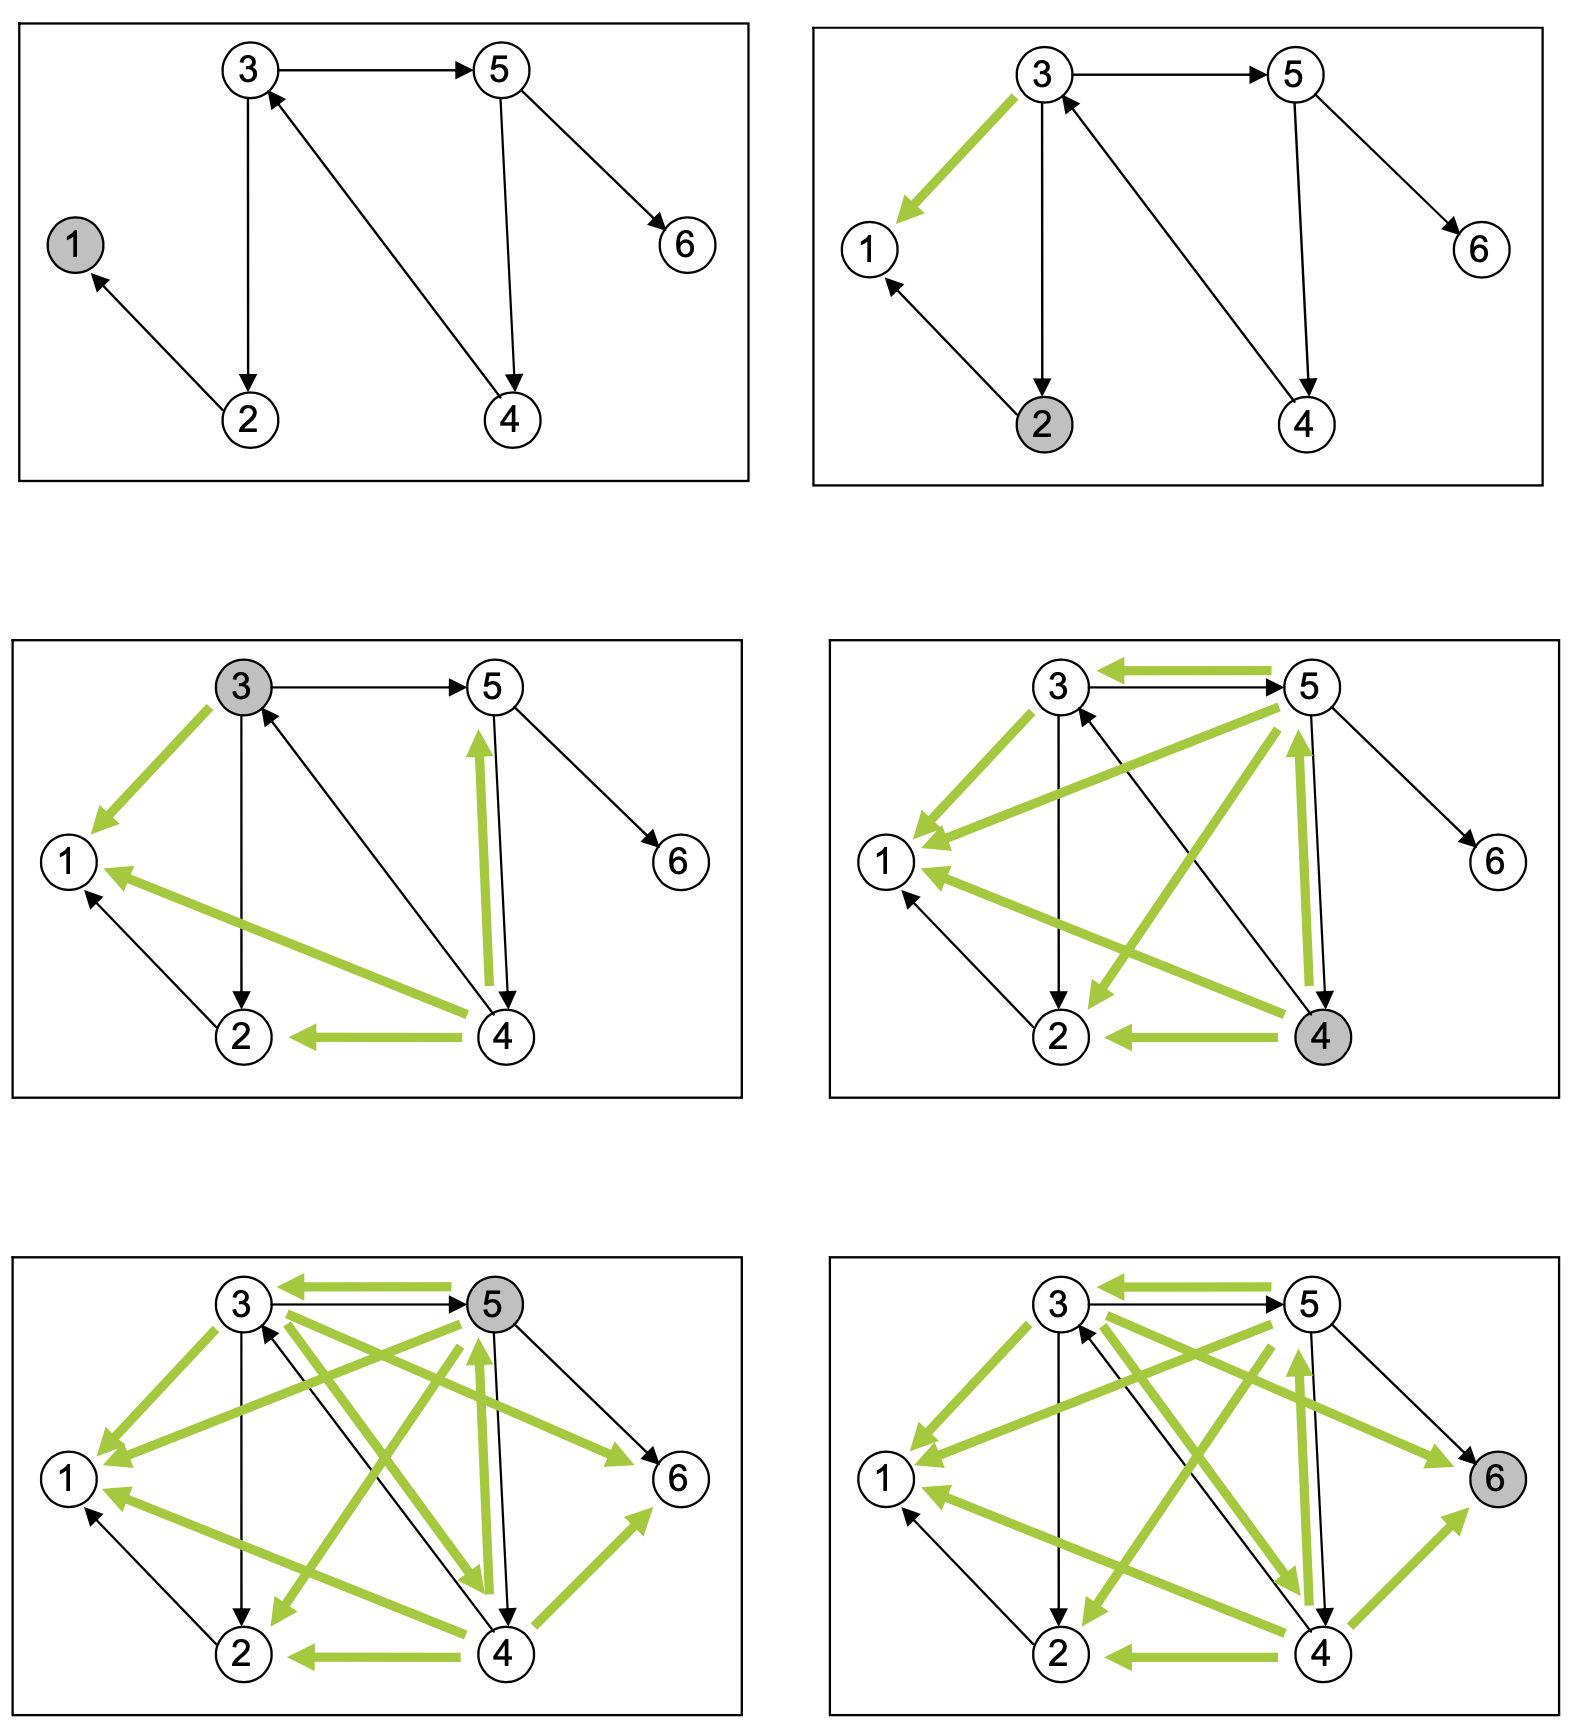
\includegraphics[scale=0.22]{14 Digraphs/Floyd-Warshall.png}
\end{center}
\newpage